\section{Metodología de Seguimiento}

Para llevar un control detallado del desarrollo del proyecto, se ha utilizado un documento en formato Excel donde se han registrado diariamente las tareas realizadas. Cada entrada incluye los siguientes campos:

\begin{itemize}\setlength{\itemsep}{0pt}
    \item \textbf{Fecha}: Fecha en la que se ha realizado la tarea.
    \item \textbf{Sección}: Categoría de la tarea (documentación, diseño, análisis...).
    \item \textbf{Tarea}: Breve descripción de la actividad llevada a cabo.
    \item \textbf{Dedicación}: Cantidad de horas empleadas dirante ese día.
    \item \textbf{Descripción}: Información más detallada sobre la tarea, incluyendo detalles relevantes que puedan ser útiles para futuras referencias.
    \item \textbf{Incidencias}: Problemas o dificultades encontradas.
    \item \textbf{Soluciones}: Posibles soluciones planteadas.
\end{itemize}

Gracias a este sistema de seguimiento, se ha podido llevar un control preciso del tiempo dedicado al proyecto y de la distribución de esfuerzos en las distintas fases. Además, con un total de 94 registros en este documento, se han podido documentar incidencias, decisiones y cambios en el alcance del proyecto, lo que ha facilitado la trazabilidad de su evolución.


\section{Materialización de Riesgos} \label{sec:materializacion_riesgos}

A lo largo del desarrollo del proyecto, se han materializado algunos de los riesgos identificados en la planificación inicial. Aunque estos riesgos afectaron de diversas formas al desarrollo, la planificación anticipada y las estrategias de mitigación permitieron minimizar sus efectos, asegurando que el TFG pudiera completarse dentro de los plazos establecidos. A continuación, se detallan los principales riesgos materializados:

\newpage

\subsection*{R01: Limitaciones con respecto a los datos disponibles de la API}

Uno de los primeros riesgos que afectaron al desarrollo del proyecto fue la disponibilidad limitada de ciertos datos en la API de \textit{Spotify}. Durante la fase inicial de validación, se comprobó que algunas de las estadísticas planteadas en la planificación no podrían implementarse debido a restricciones sobre los datos. En particular, el historial de canciones escuchadas por el usuario estaba limitado a las últimas 50 reproducciones, lo que impedía generar métricas a largo plazo.

Ante esta situación, fue necesario descartar dos de las estadísticas originales y replantear nuevas alternativas que se ajustaran a la información accesible. Este ajuste se llevó a cabo durante la primera iteración del desarrollo, en la cual se realizó un prototipado rápido para evaluar la viabilidad de distintas soluciones.

\subsection*{R02: Cambios en la política de acceso a la API}

Uno de los riesgos con mayor impacto en el proyecto fue la deprecación de varios endpoints de la API de \textit{Spotify}, anunciada el 27 de noviembre de 2024 en su blog oficial. Esta modificación inesperada obligó a replantear algunas de las estadísticas previstas, ya que varias funcionalidades dejaron de estar disponibles. En particular, la eliminación de los endpoints de \textit{Audio Features} y \textit{30-second preview URLs}, que se tomaron como base para el desarrollo.

Afortunadamente, el anuncio se realizó cuando el desarrollo se encontraba aún en una fase temprana de implementación, lo que permitió adaptar el proyecto sin afectar gravemente al progreso general. La principal acción tomada fue el rediseño de las estadísticas utilizando los datos aún accesibles en la API. Como resultado, se eliminó una de las métricas iniciales y se diseñó una nueva, siendo esta \textit{Índice de Interferencia}, presente en la implementación final.

\subsection*{R04: Incompatibilidad de versiones de las tecnologías utilizadas}

Aunque este riesgo no tuvo un impacto crítico en la funcionalidad de la aplicación, sí generó desviaciones en la planificación, especialmente en las fases de pruebas y despliegue. Se encontraron problemas de compatibilidad con ciertas dependencias a la hora de implementar las pruebas con Jest.

El mayor desafío se presentó al implementar la ejecución automática de pruebas en \textit{GitHub Actions}, donde fue necesario realizar múltiples pruebas con distintas configuraciones hasta encontrar una que funcionara correctamente. Si bien este problema supuso un retraso en el apartado de testing, no comprometió el desarrollo del resto de funcionalidades y se logró estabilizar la integración continua tras varios ajustes.

\subsection*{R06: Dificultad para compaginar el proyecto con las obligaciones académicas}

Desde el inicio del proyecto se identificó el riesgo de que la carga académica afectara al progreso del TFG, especialmente debido a la necesidad de aprobar una asignatura en diciembre para poder presentar el trabajo en febrero. Como medida preventiva, se realizó un ajuste en la distribución del tiempo de trabajo durante ese periodo, priorizando el estudio en las tres semanas previas al examen, que tuvo lugar el 16 de diciembre.

Si bien esto supuso una reducción temporal en la dedicación al TFG, la estrategia de mitigación permitió redistribuir el esfuerzo en semanas posteriores sin causar un impacto significativo en el desarrollo global del proyecto. Gracias a esta previsión, no fue necesario realizar modificaciones drásticas en los plazos generales y se pudo retomar el ritmo normal de trabajo tras el periodo de exámenes.

\section{Desviaciones en el Alcance}

A lo largo del desarrollo del proyecto, el alcance general definido en la planificación inicial se ha mantenido sin alteraciones significativas. Las funcionalidades principales, tales como la autenticación con \textit{Spotify}, el panel de información del usuario, los gráficos interactivos y la interfaz responsiva, han sido implementadas según lo previsto. Del mismo modo, las exclusiones establecidas o las limitaciones identificadas no han sufrido modificaciones.

No obstante, a nivel de funcionalidad específica, se han producido ciertos ajustes derivados de los riesgos materializados ya mencionados, que ocurrieron en los siguientes dos puntos:

\begin{itemize}
    \item \textbf{Incremento I: Prototipado Rápido}:  El riesgo \textbf{R01} se dió durante el análisis de viabilidad, se determinó que algunas estadísticas no podían implementarse debido a la falta de acceso a datos históricos de escucha.
    \item \textbf{Incremento II: Producto Mínimo Viable (PMV)}: Tras el anuncio de \textit{Spotify} sobre la deprecación de varios endpoints de su API, plevisto como el riesgo \textbf{R02}.
\end{itemize}

Como resultado de estas modificaciones, de las seis estadísticas avanzadas inicialmente previstas, cuatro han llegado a la versión final del proyecto. En la siguiente figura \ref{fig:estadisticas_cambio} se presenta el resumen de estos cambios, indicando cuáles fueron descartadas, en qué fase se produjo la decisión y los motivos que llevaron a su eliminación o sustitución.

\begin{figure}[H]
    \centering
    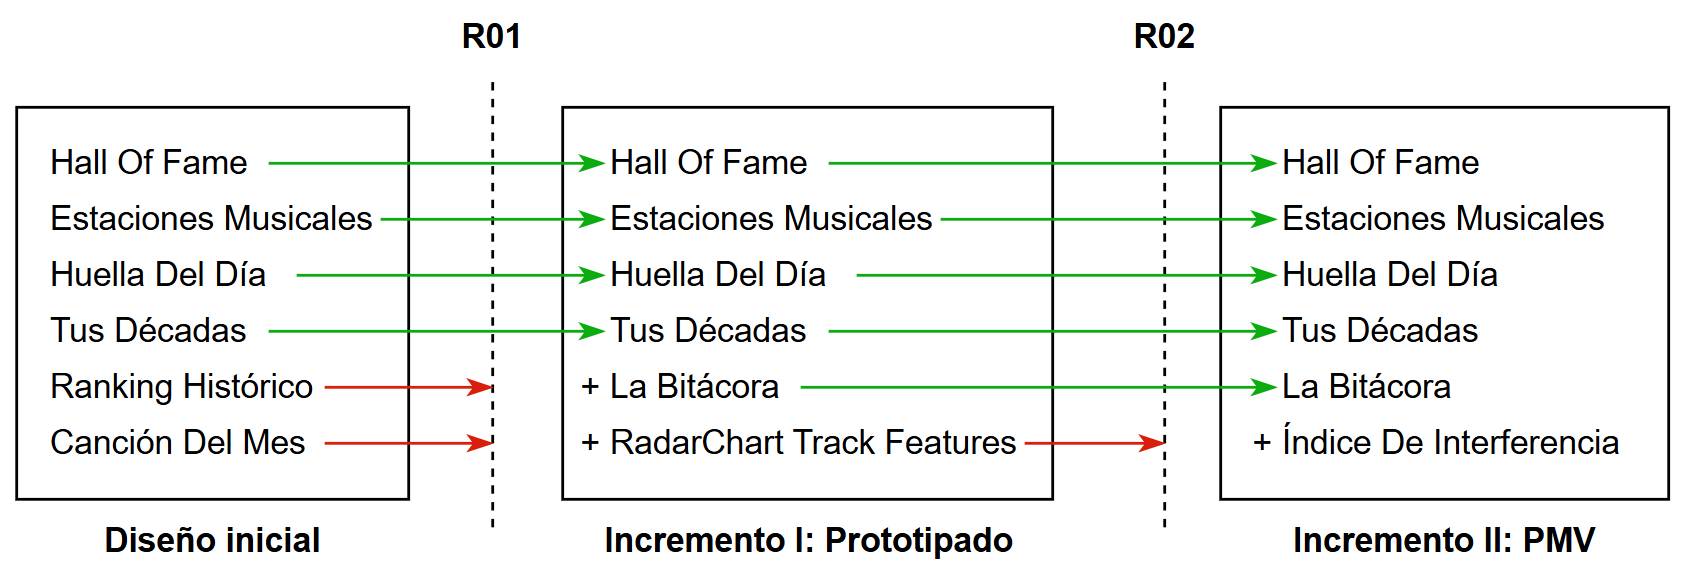
\includegraphics[width=0.9\textwidth]{figures/syc/estadisticas_cambio.png}
    \vspace{0.5cm}
    \caption{Resumen de cambios en la selección de estadísticas avanzadas.}
    \label{fig:estadisticas_cambio}
\end{figure}

\newpage

\section{Desviaciones Temporales}

A continuación, se analiza cómo las incidencias ocurridas durante el desarrollo han impactado en la planificación del proyecto desde el punto de vista temporal.

\subsection{Dedicaciones}

A lo largo del desarrollo del proyecto, las dedicaciones estimadas para cada tarea han sufrido algunas variaciones, aunque en general se han mantenido bastante alineadas con la planificación inicial. En la siguiente tabla \ref{tab:dedicaciones_real} se muestra la comparativa entre las estimaciones de dedicación establecidas en la planificación y la dedicación real registrada en el documento Excel mencionado al inicio.

\begin{figure}[H]
    \centering
    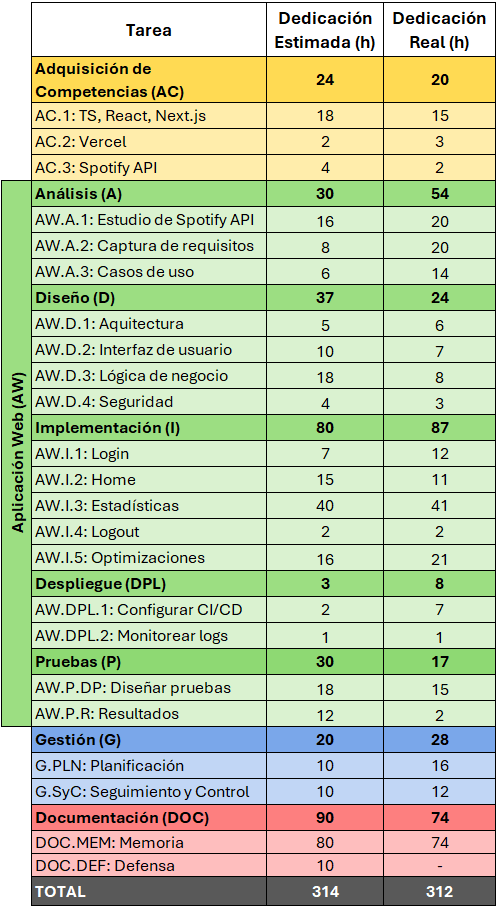
\includegraphics[width=0.6\textwidth]{figures/syc/dedicaciones_real.png}
    \vspace{0.5cm}
    \caption{Comparativa entre las dedicaciones estimadas y las reales de cada tarea.}
    \label{tab:dedicaciones_real}
\end{figure}

Aunque la dedicación total real ha sido de 312 horas, esta cifra no incluye la preparación para la defensa del TFG, ya que se llevará a cabo después de la entrega de esta memoria. Teniendo en cuenta este aspecto, la \textbf{dedicación real se aproximará más a las 320 horas}, un valor ligeramente superior a lo planificado.

Sin embargo, el hecho de que la suma total de horas sea similar a la prevista no significa que no haya habido desviaciones significativas en tareas individuales, sino que estas han terminado compensándose entre sí. A continuación, se analiza en detalle los principales puntos de desviación y las razones que los han provocado:

\begin{itemize}
    \item \textbf{Análisis (A)}: Se observa un incremento notable en la dedicación a este apartado debido a la decisión de realizar un prototipado inicial de las estadísticas, lo cual se ha incluido dentro de esta fase.
    \item \textbf{AW.D.2 y AW.D.3}: La menor dedicación en estas tareas se debe a que gran parte del diseño de la interfaz y la lógica se llevó a cabo durante la construcción del PMV en la fase de implementación. Como consecuencia, en la fase de diseño solo fue necesario plasmar las decisiones que ya se habían tomado durante el segundo incremento de la aplicación.
    \item \textbf{AW.I.1}: La implementación del \textit{Login} de la web se alargó debido a que era la primera funcionalidad que se implementaba, por lo que no se estaba del todo familiarizado con las tecnologías como \textit{Next.js} y \textit{TypeScript}, lo que llevó a varias correcciones tras la primera implementación.
    \item \textbf{AW.I.5}: Dentro de la tarea de Optimizaciones se ha incluido el desarrollo del tercer incremento de la aplicación, que resultó una tarea mayor de lo que inicialmente representarían.
    \item \textbf{Despliegue (DPL)}: Este apartado incluye la configuración de \textit{GitHub Actions}, la cual generó diversas complicaciones, como ya se ha detallado en el apartado de \nameref{sec:materializacion_riesgos}.
    \item \textbf{Pruebas (P)}: La considerable reducción en las horas dedicadas se debe principalmente a la tarea AW.P.R, donde se había previsto un mayor número de errores. Al realizar la planificación con márgenes laxos, se estimo un tiempo amplio si ocurría el caso de la aparición de muchos errores.
    \item \textbf{Documentación (DOC)}: La reducción en la dedicación a esta tarea es únicamente aparente, ya que no se han contabilizado las horas correspondientes a la tarea DOC.DEF, relativa a la preparación de la defensa.
\end{itemize}

\newpage

\subsection{Plazos del Desarrollo}

En cuanto a los plazos generales, ha habido algunos ajustes en la distribución temporal de las tareas. La mayor desviación se produjo en diciembre, cuando el desarrollo del TFG se paralizó durante tres semanas debido a la preparación del examen de la asignatura. Esta interrupción tuvo un impacto en el calendario de desarrollo, pero las tareas fueron reubicadas en los meses siguientes sin que ello generara problemas significativos. Gracias a la flexibilidad de la planificación, estas variaciones pudieron absorberse sin afectar la fecha final de entrega.

\begin{figure}[H]
    \centering
    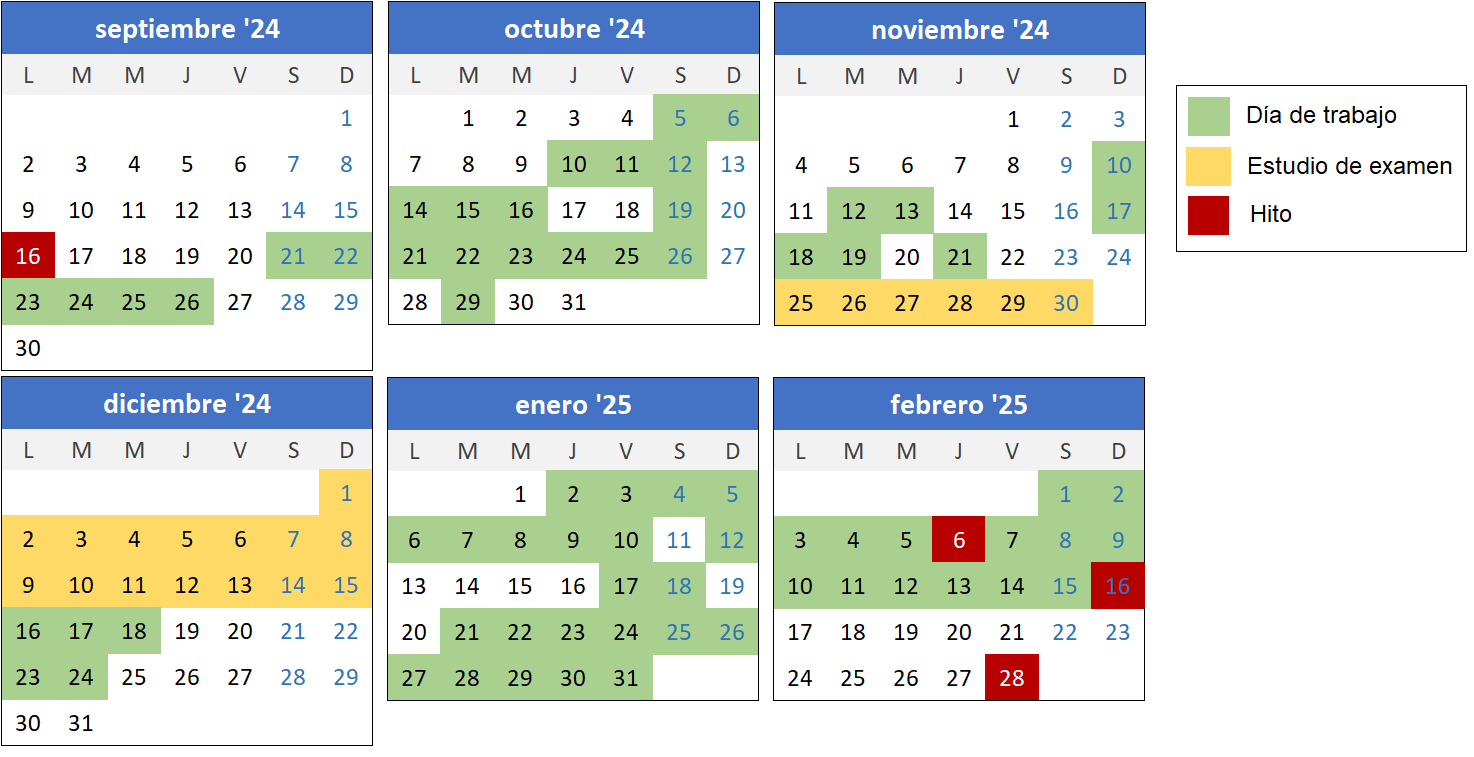
\includegraphics[width=0.9\textwidth]{figures/syc/calendario_trabajo.png}
    \vspace{0.5cm}
    \caption{Canlendario indicando los días de trabajo realizados, el periodo de examen y fechas de hitos}
    \label{tab:calendario_trabajo}
\end{figure}


Otro de los cambios mencionables en la planificación fue la evolución del ciclo de desarrollo de la aplicación. Inicialmente, se había planteado un enfoque más lineal, pero con el avance del proyecto se decidió adoptar un modelo incremental. Para garantizar un mejor análisis y diseño del sistema, se creó un \textbf{Producto Mínimo Viable (PMV)}. Aunque esta decisión no estaba prevista desde el inicio, surgió de manera orgánica durante el proceso y resultó beneficiosa para el desarrollo.

Más allá de estas adaptaciones, el desarrollo del proyecto se ha mantenido dentro de los plazos previstos, permitiendo completar todas las fases necesarias sin desviaciones críticas.

\section{Revisión de Objetivos}

El desarrollo del proyecto ha concluido con éxito, logrando cumplir plenamente con los objetivos planteados en la fase inicial. El \textbf{objetivo general} se ha alcanzado de manera satisfactoria, que consistía en desarrollar una plataforma web interactiva que permitiera a los usuarios de \textit{Spotify} acceder a visualizaciones y análisis de sus datos musicales personales.

Además del objetivo general, cada uno de los \textbf{objetivos específicos} establecidos en la planificación también ha sido cumplido con éxito:

\newpage

\begin{itemize}
    \item \textbf{Análisis de la API de Spotify}: Parte fundamental del proyecto, se identificaron las restricciones y posibilidades de la API.
    \item \textbf{Procesamiento de datos}: Se implementó la lógica necesaria para filtrar, organizar y transformar los datos obtenidos en el backend de la aplicación mediante los \textit{Route Handlers}.
    \item \textbf{Diseño de la interfaz de usuario}: Gracias a la facilidad de uso de los estilos de \textit{Tailwind CSS}, se desarrolló una interfaz intuitiva, interactiva y responsiva, asegurando una experiencia de usuario fluida en distintos dispositivos.
    \item \textbf{Uso de tecnologías modernas}: Se utilizaron \textit{Next.js}, \textit{React} y \textit{TypeScript}, aprovechando sus ventajas en estructuración del código, tipado estático y rendimiento optimizado.
    \item \textbf{Automatización del despliegue}: Se implementaron prácticas de \textit{CI/CD} con \textit{Vercel} y \textit{GitHub Actions}, permitiendo un flujo automatizado de pruebas antes de un despliegue, accionado por un push a la rama principal \texttt{main}.
    \item \textbf{Seguridad y gestión de datos}: Se respetaron las políticas de \textit{Spotify} relevantes para este proyecto, como la no persistencia de datos, la gestión de la autorización mediante \textit{OAuth 2.0} y el manejo seguro de los datos del usuario.
    \item \textbf{Documentación del desarrollo}: Se registró detalladamente el proceso completo, asegurando la trazabilidad de las decisiones y facilitando la revisión del trabajo realizado, plasmado en esta memoria.
\end{itemize}

En conclusión, el proyecto \textbf{ha cumplido con éxito todos sus objetivos}, tanto a nivel general como en cada uno de los aspectos específicos definidos en la planificación. A pesar de algunos ajustes en funcionalidades concretas debido a limitaciones técnicas, la plataforma desarrollada mantiene la esencia del planteamiento original y proporciona una experiencia completa y funcional para el usuario.
